\subsection{Activating the pump}\label{subsec:activating-the-pump}

The next requirement is to distribute the formic acid.
In this requirement, a pump must be controlled, that is transferring the acid from a storage container to the bee hive.
This has to be done once per hour, with a variable amount of fluid depending on the temperature.
How the temperature is measured and the volume selected is already shown in section \ref{subsec:reading-temperature}.

This requirement is implement similarly to how the fan is controlled in section \ref{subsec:activating-the-fan}.
A relay is used to control if the circuit, between the powerbank and the pump, is open or closed.
Each hour the circuit is closed, activating the pump.
The circuit stays closed until the pump has delivered the necessary amount of formic acid.
Then the circuit is opened again, deactivating the pump.

\begin{lstlisting}[label={lst:pump-control},language=C++, caption=Controling the pump]
void loop() {
    ...
    if (millis() - lastPumpCycle >= ONE_HOUR) {
        ...
        getPump()->start(millis());

        while(mustContinuePumping(lastSensorReadings.temperature)) {
            delay(100);
        }
        ...
            getPump()->stop();
        ...
        lastPumpCycle = millis();
    }
}
\end{lstlisting}

Listing \ref{lst:pump-control} shows this process in more detail.
First the time between the current time and the time of the last pump cycle is measured.
If this timespan is equal or greater to one hour, the pump is started.
As long as the pump has not delivered enough fluid, the program is halted for 100 millisecond, after which this state is determined again.
The method \textit{mustContinuePumping} is explain in section \ref{subsec:reading-temperature}.
When the pump must stop, the loop exits, the program continues and stops the pump.

\begin{figure}
    \centering
    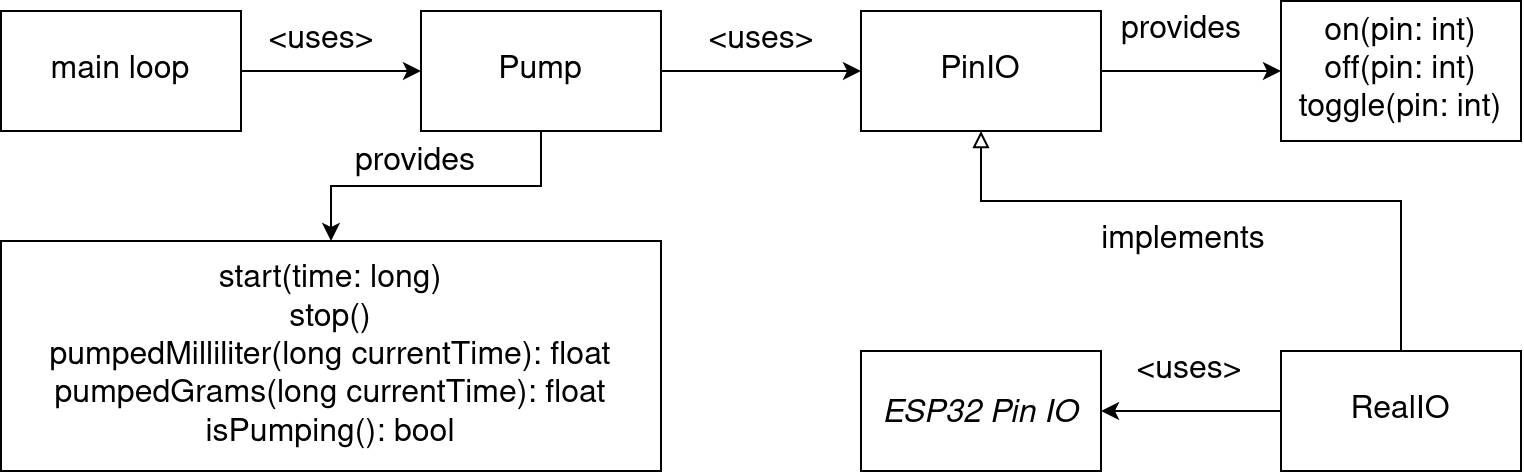
\includegraphics[width=\textwidth]{img/pump-control}
    \caption{Abstraction of the pump control}
    \label{fig:abstraction-of-pump}
\end{figure}

Since controlling the pump necessitates knowledge about its flow rate and how long it is running, the behaviour is more abstracted.
This abstraction is visualized in Figure \ref{fig:abstraction-of-pump}.
Instead of the main loop using the \textit{PinIO} interface directly, it is used by a \textit{Pump} class.
This class encapsulates all the necessary methods, such as \textit{start} and \textit{stop}.
It also stores the time when it was started, to calculated how much acid was delivered when the methods \textit{pumpedMilliliter} or \textit{pumpedGrams} are called.
The method \textit{isPumping} returns true if the pump was started and not stopped, or false otherwise.